\subsection{The ESDM Configuration File}

%\begin{figure}
%  \centering
%  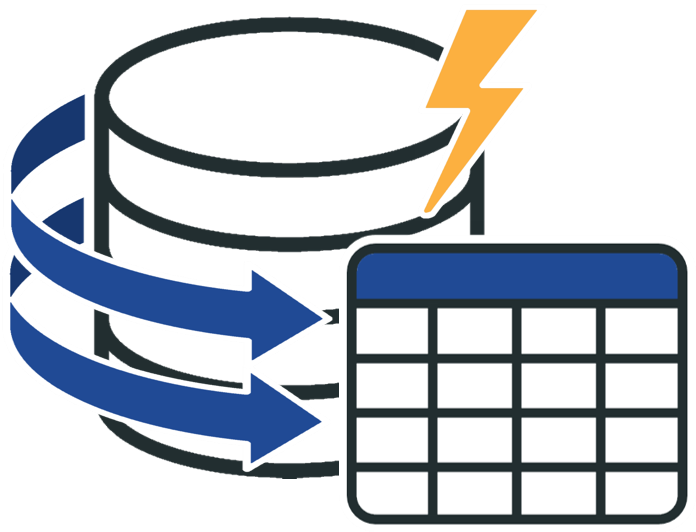
\includegraphics[width=0.9\textwidth]{figures/data-model.png}
%  \caption{Dummy figure}
%  \label{fig:dummy}
%\end{figure}

\subsubsection{Search Paths}

TODO

\subsubsection{File Format}

The configuration file format is based on JSON, i.e. all configuration files must be valid JSON files.
However, ESDM places some restrictions on what keys are recognized and which types are expected.
The tables summarize parameters that can be used in the configuration file.
Parameter can be of four types: string, integer, float and object, which are collections of key-value pairs.

The ```"esdm":{}``` key-value pair in the root of the JSON configuration file can contain configuration for multiple data backends and one metadata backend.
The backends are organized in the ```backends``` key-value pair as a list.

\begin{lstlisting}
{
  "esdm":	{
    "backends": [backend_1, backend_2, \ldots, backend_n],
    "metadata": {}
  }
}
\end{lstlisting}


\begin{table}[!h]
  \centering
  \begin{tabularx}{\textwidth}{llllX}
  Parameter              & Type    & Default    &          & Description \\
  \hline
  type                   & string  & (not set)  & required & Backend name (see \Cref{tab:supported_backends}) \\
  id                     & string  & (not set)  & required & Unique identifier string \\
  target                 & string  & (not set)  & required & Connection specification (Bucket name for S3) \\
  performance-model      & object  & (not set)  & optional & Performance model definition. (see \Cref{tab:dyn_perf_model_conf_params,tab:gen_perf_model_conf_params}) \\
  max-threads-per-node   & integer & 0          & optional & Maximum number of threads on a node. \\
  write-stream-blocksize & integer & 0          & optional & TODO. \\
  max-global-threads     & integer & 0          & optional & Maximum total number of threads. \\
  accessibility          & string  & global     & optional & TODO. (see \Cref{tab:accessibility}) \\
  max-fragment-size      & integer & 10485760   & optional & Maximum fragment size in bytes. \\
  fragmentation-method   & string  & contiguous & optional & Fragmentation methods. (see \Cref{tab:frag_methods}) \\
  % S3 parameters
  host                   & string  & (not set)  & required & (S3 only) TODO \\
  secret-key             & string  & (not set)  & required & (S3 only) TODO \\
  access-key             & string  & (not set)  & required & (S3 only) TODO \\
  locationConstraint     & string  & (not set)  & required & (S3 only) TODO \\
  authRegion             & string  & (not set)  & required & (S3 only) TODO \\
  timeout                & integer & (not set)  & required & (S3 only) TODO \\
  s3-compatible          & integer & (not set)  & required & (S3 only) TODO \\
  use-ssl                & integer & 0          & required & (S3 only) TODO \\
  \end{tabularx}
  \caption{Backend configuration parameters}%
  \label{tab:backend_conf_params}
\end{table}




\paragraph{Parameter: id}
Unique identifier string.


\paragraph{Parameter: type and target}
Can take a value of one of the supported backends listed in @tbl:supportedtypes.

\begin{table}[!h]
  \centering
  \begin{tabular}{ll}
    Type   & Description                     \\ 
    \hline
    CLOVIS & Seagate Object Storage API      \\ 
    DUMMY  & (Used for development)          \\ 
    IME    & DDN Infinite Memory Engine      \\ 
    KDSA   & Kove Direct System Architecture \\ 
    POSIX  & POSIX interface                 \\ 
    S3     & Amazon Simple Storage Service   \\ 
    WOS    & DDN Object Storage              \\ 
  \end{tabular}
  \caption{Supported backends}%
  \label{tab:supported_backends}
\end{table}

\subparagraph{type = MOTR}

\begin{lstlisting} 
[local_addr] [ha_addr] [prof] [proc_fid]
\end{lstlisting}

  where
  \begin{itemize}
    \item "local\_addr" is the local address used to connect to Motr service, 
    \item "ha\_addr" is the hardware address in Motr service, 
    \item "prof" is the profile FID in the Motr service, and
    \item "proc\_fid" is the process FID in the Motr service.
  \end{itemize}
  
  \begin{lstlisting} 
  {
   "type": "MOTR",
   "id": "c1",
   "target": ":12345:33:103 192.168.168.146@tcp:12345:34:1 
     <0x7000000000000001:0> <0x7200000000000001:64>"
  }
  \end{lstlisting}
        
\subparagraph{type = DUMMY}

(Used for development)

\subparagraph{type = IME}
  TODO

  \begin{lstlisting}
  {
   "type": "IME",
   "id": "p1",
   "target": "./_ime"
  }
  \end{lstlisting}

\subparagraph{type = KDSA}

Prefix ``xpd:'' followed by volume specifications. Multiple volume names can be connected by ``+'' sign.

\begin{lstlisting}
xpd:mlx5\_0.1/260535867639876.9:e58c053d-ac6b-4973-9722-cf932843fe4e[+mlx...]
\end{lstlisting}

A module specification consists of several parts.
Caller provides a device handle, the target serial number, the target link number, the volume UUID,
The convention for specifying a KDSA volume uses the following format:

\begin{lstlisting}
[localdevice[.localport]/][serialnumber[.linknum]:]volumeid
\end{lstlisting}

where the square brackets indicate optional parts of the volume connection specification.
Thus, a volumeid is nominally sufficient to specify a desired volume, and one can then optionally additionally 
specify the serial number of the XPD with optional link number, and/or one can optionally specify the local 
device to use with optional local port number.
The convention for specifying multiple KDSA volumes to stripe together uses the following format:

\begin{lstlisting}
volume_specifier[+volume_specifier[+volume_specifier[+...]]][@parameter]
\end{lstlisting}

where the square brackets indicate optional parts of the aggregated connection specification. Thus, a single
volume connection specification is sufficient for a full connection specifier, and one can then optionally specify
additional volume specifiers to aggregate, using the plus sign as a separator. The user may also additionally
specify parameters for the aggregation, using the “at sign”, a single character as a parameter identifier, and the
parameter value.

\begin{lstlisting}
{
"type": "KDSA",
"id": "p1",
"target": "This is the XPD connection string",
"max-threads-per-node" : 0,
"max-fragment-size" : 1048,
"accessibility" : "global"
}
\end{lstlisting}

\subparagraph{POSIX}

Path to a directory, e.g., /home/user/data/

\begin{lstlisting}
{
 "type": "POSIX",
 "id": "p2",
 "target": "./_posix2"
}
\end{lstlisting}

\subparagraph{S3}
Bucket name prefix (at least 5 characters long)

\begin{table}[!h]
  \centering
  \begin{tabularx}{\textwidth}{llllX}
  Parameter              & Type    & Default    &          & Description \\
  \hline
  host                   & string  & (not set)  & required & (S3 only) TODO \\
  secret-key             & string  & (not set)  & required & (S3 only) TODO \\
  access-key             & string  & (not set)  & required & (S3 only) TODO \\
  locationConstraint     & string  & (not set)  & required & (S3 only) TODO \\
  authRegion             & string  & (not set)  & required & (S3 only) TODO \\
  timeout                & integer & (not set)  & required & (S3 only) TODO \\
  s3-compatible          & integer & (not set)  & required & (S3 only) TODO \\
  use-ssl                & integer & 0          & required & (S3 only) TODO \\
  \end{tabularx}
  \caption{S3 parameters}%
  \label{tab:s3_params}
\end{table}

TODO example

\subparagraph{WOS}
TODO

\begin{lstlisting}
{
"type": "WOS",
"id": "w1",
"target": "host=192.168.80.33;policy=test;",
"max-threads-per-node" : 1,
"max-fragment-size" : 1073741825,
"max-global-threads" : 1,
"accessibility" : "global"
}
\end{lstlisting}


\subparagraph{Parameter: performance-model}


\begin{table}[!ht]
  \centering
  \begin{tabularx}{\textwidth}{lllllX}
    Parameter  & Type  & Default & Domain &          & Description \\ 
    \hline
    latency    & float & 0.0     & >=0.0  & optional & seconds     \\ 
    throughput & float & 0.0     & >0.0   & optional & MiB/s       \\ 
  \end{tabularx}
  \caption{Dynamic performance model parameters}%
  \label{tab:dyn_perf_model_conf_params}
\end{table}


\begin{table}[!ht]
  \centering
  \begin{tabularx}{\textwidth}{lllllX}
    Parameter  & Type    & Default & Domain &          & Description         \\ 
    \hline
    latency    & float   & 0.0     & >=0.0  & optional & Latency in seconds  \\ 
    throughput & float   & 0.0     & >0.0   & optional & Throughput in MiB/s \\ 
    size       & integer & 0       & >0     & optional & TODO                \\ 
    period     & float   & 0.0     & >0.0   & optional & TODO                \\ 
    alpha      & float   & 0.0     & [0.0,  & 1.0)     & optional TODO       \\ 
  \end{tabularx}
  \caption{Generic performance model parameters}%
  \label{tab:gen_perf_model_conf_params}
\end{table}



\subparagraph{Parameter: max-threads-per-node}
TODO

\subparagraph{Parameter: write-stream-blocksize}
TODO

\subparagraph{Parameter: max-global-threads}
TODO

\subparagraph{Parameter: accessibility}

\begin{table}[!ht]
  \centering
  \begin{tabularx}{\textwidth}{lX}
    Method & Description \\ 
    \hline
    global & TODO        \\ 
    local  & TODO        \\ 
  \end{tabularx}
  \caption{Accessibility}%
  \label{tab:accessibility}
\end{table}

\subparagraph{Parameter: max-fragment-size}
The amount of data that may be written into a single fragment. 
The amount is given in bytes.

\subparagraph{Parameter: fragmentation-method}
A string identifying the algorithm to use to split a chunk of data into fragments. 
Legal values are:

\begin{table}[!ht]
  \centering
  \begin{tabularx}{\textwidth}{lX}
Method     & Description \\
\hline
contiguous  & This algorithm tries to form fragments that are 
            scattered across memory as little as possible. As such, 
            it is expected to yield the best possible write performance. 
            However, if a transposition is performed when reading 
            the data back, performance may be poor.
            Splitting a dataspace of size (50, 80, 100) into fragments 
            of 2000 entries results in fragments of size (1, 20, 100). \\
equalized   & This algorithm tries to form fragments that have a similar 
            size in all dimensions. As such, it is expected to perform 
            equally well with all kinds of read requests, but it tends 
            to write scattered data to disk which has to be sequentialized 
            first, imposing a performance penalty on the write side.
            Splitting a dataspace of size (50, 80, 100) into fragments of at
            most 2000 entries results in fragments of sizes between 
            (10, 11, 11) and (10, 12, 12). \\
  \end{tabularx}
  \caption{Fragmentation methods}%
  \label{tab:frag_methods}
\end{table}


\subsubsection{Metadata}%
\label{sec:conf-file:metadata}

\begin{table}[!ht]
  \centering
  \begin{tabularx}{\textwidth}{lllX}
    Parameter & Type   & Default   & Description     \\ 
    \hline
    type      & string & (not set) & required TODO   \\ 
    id        & string & (not set) & (not used) TODO \\ 
  \end{tabularx}
  \caption{Metadata parameters}%
  \label{tab:metadata_params}
\end{table}

